\documentclass[a4paper]{article}

\usepackage[english]{babel}
\usepackage[utf8]{inputenc}
\usepackage{apacite}
\usepackage{graphicx}
\usepackage{tikz}
\usetikzlibrary{positioning}
\usepackage{xcolor}
\usepackage[colorinlistoftodos]{todonotes}

\makeatletter
\def\BState{\State\hskip-\ALG@thistlm}
\makeatother

\title{Gameplay Design \\ Assignment 2 }

\author{
  Bowald, Johan\\
  \texttt{bowaldj@student.chalmers.se}
  \and
  Odbjer, Sebastian\\
  \texttt{sebastian.odbjer@gmail.com}
}

\date{\today}

\tikzset{
    vertex/.style = {
        circle,
        fill  = black,
        outer sep = 2pt,
        inner sep = 1pt,
    }
}

\begin{document}
\maketitle
\newpage
\tableofcontents{}
\newpage
\section{Introduction}

\section{Gameplay description 7 wonders}
\label{sec:what7wond}
7 wonder was released in 2010 and the goal is to build a civilisation in an ancient setting. 
The game consist of several card types and a player unique game board showing the status of a players civilisation. The different cards represents different buildings which each contribute to the civilisation in some way. There are resource spawning, such as iron, chemicals or wood. Military cards which are used to battle with one's neighbours, these battles gives points to the victor and minus point to the defeated one. Battles is Science Cards, which generate points at the end of the game, the amount of points is based on the amount of science tool sets collected and the number of each science tool.
Another card type is what we have called utility cards, they have an immediate effect on the game state, these are cards that either is tradeable for currency or trading posts that gives discount for trading with one's neighbours. Last card type is point cards, either buildings that gives a fixed amount of points or dynamic point cards that is based on oneself civilisation status or ones neighbours statuses. The game is divided into three ages, each age is divided into six turns. Each turn, each player picks a card which is either played, discarded or used as a resource to build a wonder. The rest of the cards is passed to the next player in a drafting fashion. To play a card some resources must be paid, they can either be resources generated Wonders have different impact on the game, they can either generate resources, points, currency or military power. The effect of wonders are unique for each civilisation. After the three ages points are counted for each player based on each card type, and the amount of currency when the game is over. The player that has the most point at the end wins the game. 

\subsection{Thoughts on gameplay of 7 wonders}
\label{sec:thoughtsGP7wond}
\paragraph{The gameplay in this game} is centered around the draft mechanic. A player will always consider which strategy to use based on his neighbours choice of card, what resources they have, status of their military power and or their ability to trade cheap resources to them self. 

\citeauthor{critical7wond} makes a statement about the scalability of players in the game. That even if this game can scale up to seven players. One is mostly affected by its neighbours. Thou arguing for 2-3 players being the optimal to play. Because this tightens the gameplay. 
7 wonders can be played with two to seven player. Boardgamegeeks suggest that its best with four players. The argument is that since each player only can have two neighbors. We have tried to play the game with three players and five players. When plaing with many player we can agree with \citeauthor{critical7wond} that one feels distant with players that are not neighbours. But in a game of three a player have more information of which cards that are in the draft pool and have more information. Thus playing with more then three player is more fun in our opinion.

\citeauthor{opiogamers7wond} makes an argument about the drafting design of the game. That even if a player makes a lot of decision. Most of these descisions dont matter in the end it is about to find the "perfect card" at the right time more then the previous decisions. Our thoughts about this is even if that is the case this is the nature of the \textit{drafting} mechanich. Also to get in the spot of the getting the perfect card one has to make decisions so that one minimize the possiblity that a oppnent need the same "perfect card" as oneself.



\section{Gameplay description Ricocheting Robots}
Ricochet robots is a game where players challenge each other to move a robot to a certain point.. The game consists of a board with a grid layout. Some of the grid tiles are unique goal tile. The goal tiles have a color matching one of the robots(except the optional support robot) and a symbol. The board also have walls placed between some tiles. A robot cannot move through these walls, instead they ricochet along the wall in the direction of the players choice. Each turn a goal token is revealed and each player simentainusly tries to figure out the path with the fewest moves to take the robot with the matching color as the goal token to the goal tile with the same symbol and color as the goal token. 

, with the goal of move a specific robot from one point to a goal point. When one player have found a legit path, that player state the amount of movements required to carry out the task. The other players have one minute to try to beat the first player number of movements. When the time ends, that player with the fewest movements gets the point and a new turn begins. When all goal tokens are collected by the players, the player with the most goal tokens wins the game.

\section{Analysis using game design patterns}
We have analize using Game Design patterns framework /cite{Bjork2003}. Some of the patterns is fetch from the wikipedia for Gameplay Design Patterns \url{gdp2.tii.se}. Others is defined by us. At the end of this section a comparison of both games is presented.

\newpage
\subsection{7 wonders analysis}
\begin{figure}[htb]

\centering
  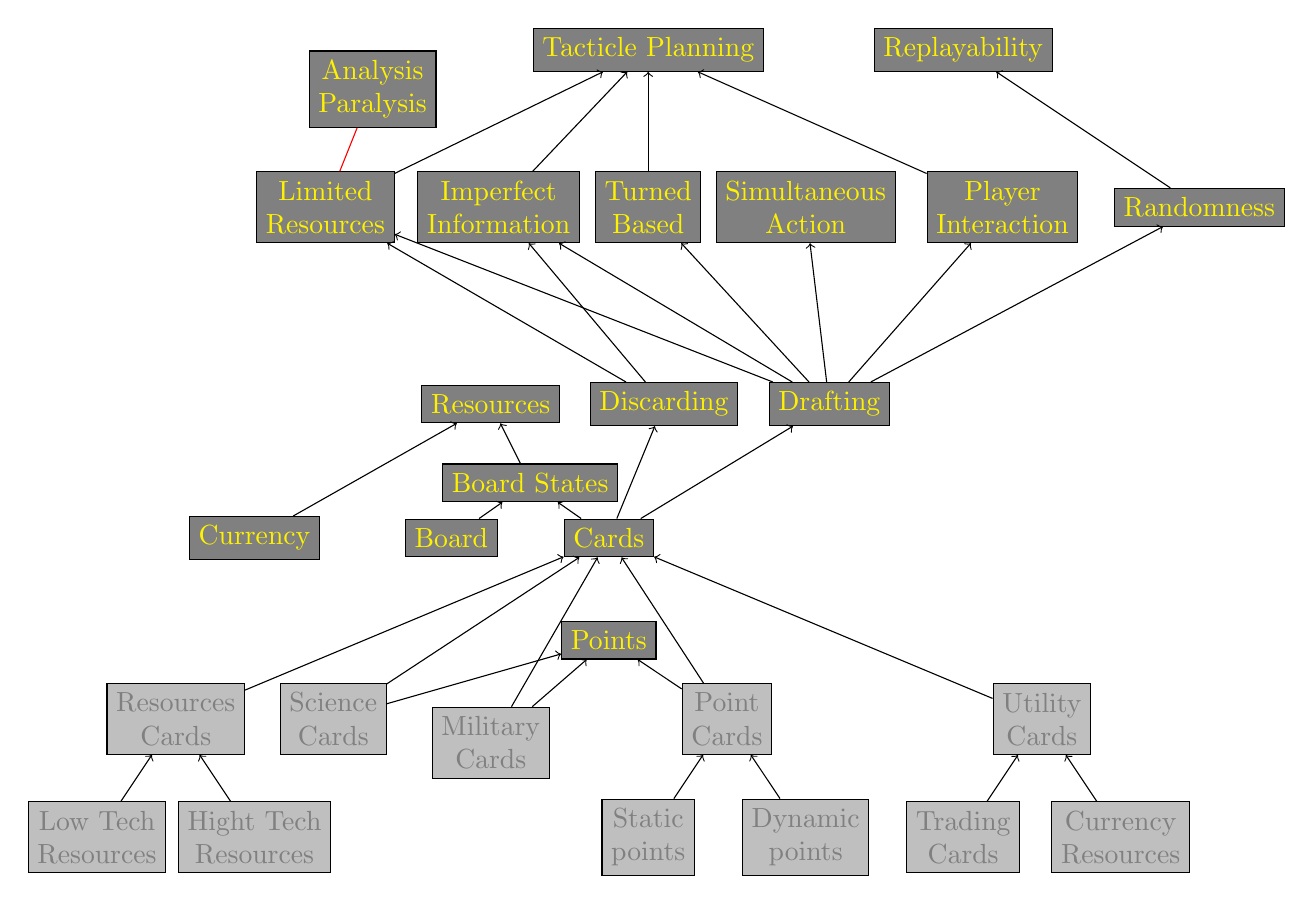
\begin{tikzpicture}

  \node[draw,fill=gray!50,text=gray, align=center] (LTRe) at (-6,0) {Low Tech\\ Resources};
  \node[draw,fill=gray!50,text=gray, align=center] (HTRe) at (-4,0){Hight Tech\\ Resources};

  \node[draw,fill=gray!50,text=gray, align=center] (CuRe) at (7,0) {Currency \\Resources};
  \node[draw,fill=gray!50,text=gray, align=center] (TrCa) at (5,0) {Trading \\Cards};  

  \node[draw,fill=gray!50,text=gray, align=center] (StPo) at (1,0) {Static\\points};
  \node[draw,fill=gray!50,text=gray, align=center] (DyPo) at (3,0) {Dynamic\\points};
  
  \node[draw,fill=gray!50,text=gray, align=center] (ReCa) at (-5,1.5) {Resources\\ Cards};
  \draw[->,draw=black] (LTRe) to (ReCa);
  \draw[->,draw=black] (HTRe) to (ReCa);
  \node[draw,fill=gray!50,text=gray, align=center] (ScCa) at (-3,1.5) {Science\\Cards};
  \node[draw,fill=gray!50,text=gray, align=center] (MiCa) at (-1,1.2) {Military\\Cards};
  \node[draw,fill=gray!50,text=gray, align=center] (PoCa) at (2,1.5) {Point\\Cards};
  \draw[->,draw=black] (DyPo) to (PoCa);
  \draw[->,draw=black] (StPo) to (PoCa);
  \node[draw,fill=gray!50,text=gray, align=center] (UtCa) at (6,1.5) {Utility\\Cards};
  \draw[->,draw=black] (TrCa) to (UtCa);
  \draw[->,draw=black] (CuRe) to (UtCa);

  \node[draw,fill=gray,text=yellow] (Po) at (0.5,2.5) {Points};

  \draw[->,draw=black] (ScCa) to (Po);
  \draw[->,draw=black] (MiCa) to (Po);
  \draw[->,draw=black] (PoCa) to (Po);

  \node[draw,fill=gray,text=yellow] (Ca) at (0.5,3.8) {Cards};

  \draw[->,draw=black] (ScCa) to (Ca);
  \draw[->,draw=black] (MiCa) to (Ca);
  \draw[->,draw=black] (PoCa) to (Ca);
  \draw[->,draw=black] (ReCa) to (Ca);
  \draw[->,draw=black] (UtCa) to (Ca);
  
  % \node[draw,fill=gray!50,text=gray, align=center ](PoTo) {Point\\Tokens};
  \node[draw,fill=gray,text=yellow] (Cu) at (-4,3.8){Currency};
  \node[draw,fill=gray,text=yellow] (Bo) at (-1.5,3.8){Board};


  % %to points, resouces
  \node[draw,fill=gray,text=yellow] (BoSt) at (-0.5,4.5) {Board States};
  \draw[->,draw=black] (Bo) to (BoSt);
  \draw[->,draw=black] (Ca) to (BoSt);

  \node[draw,fill=gray,text=yellow] (Re) at (-1,5.5) {Resources};
  \node[draw,fill=gray,text=yellow] (Di) at (1.2,5.5) {Discarding};
  \node[draw,fill=gray,text=yellow] (Da) at (3.3,5.5) {Drafting};
  \draw[->,draw=black] (Cu) to (Re);
  \draw[->,draw=black] (BoSt) to (Re);
  \draw[->,draw=black] (Ca) to (Da);
  \draw[->,draw=black] (Ca) to (Di);

  % %Drafting, discarding
  \node[draw,fill=gray,text=yellow, align=center] (ImIn) at (-0.9,8) {Imperfect\\Information};
  \node[draw,fill=gray,text=yellow, align=center] (LiRe) at (-3.1,8) {Limited\\Resources};
  \node[draw,fill=gray,text=yellow, align=center] (TuBa) at (1,8) {Turned\\Based};
  \node[draw,fill=gray,text=yellow, align=center] (SiAc) at (3,8) {Simultaneous\\Action};
  \node[draw,fill=gray,text=yellow, align=center] (PlIn) at (5.5,8) {Player\\Interaction};
  \node[draw,fill=gray,text=yellow, align=center] (Ra) at (8,8) {Randomness};

  \draw[->,draw=black] (Di) to (ImIn);
  \draw[->,draw=black] (Di) to (LiRe);

  \draw[->,draw=black] (Da) to (ImIn);
  \draw[->,draw=black] (Da) to (LiRe);
  \draw[->,draw=black] (Da) to (TuBa);
  \draw[->,draw=black] (Da) to (SiAc);
  \draw[->,draw=black] (Da) to (PlIn);
  \draw[->,draw=black] (Da) to (Ra);

  % %Drafting trading cards
  
  \node[draw,fill=gray,text=yellow, align=center] (AnPa) at (-2.5,9.5){Analysis\\Paralysis};
  \draw[-,draw=red] (LiRe) to (AnPa);
  \node[draw,fill=gray,text=yellow] (TaPl) at (1,10){Tacticle Planning};
  \node[draw,fill=gray,text=yellow] (Re) at (5,10){Replayability};
  \draw[->,draw=black] (ImIn) to (TaPl);
  \draw[->,draw=black] (LiRe) to (TaPl);
  \draw[->,draw=black] (TuBa) to (TaPl);
  \draw[->,draw=black] (PlIn) to (TaPl);
  \draw[->,draw=black] (Ra) to (Re);

  % \node[draw,fill=gray,text=yellow] (KiMa) {King Maker};

  \end{tikzpicture}
\caption{Analysis of 7 Wonders using Game Design Pattern. Light gray boxes indicates gameplay mechanics unique to 7 wonders. Dark gray boxes ate abstract mechanics found in other games. Edges with arrows indicate that the pattern being pointed to is instantiated by the other pattern connected to the edge. Red edges indicates that at pattern is in conflict with another pattern.}
\label{fig:A7W}
\end{figure}

\newpage
\subsection{Ricocheting Robots analyzed using Game Design Patterns}
% Ricocheting Robots Game pattern analysis
\begin{figure}[htb]
\centering
  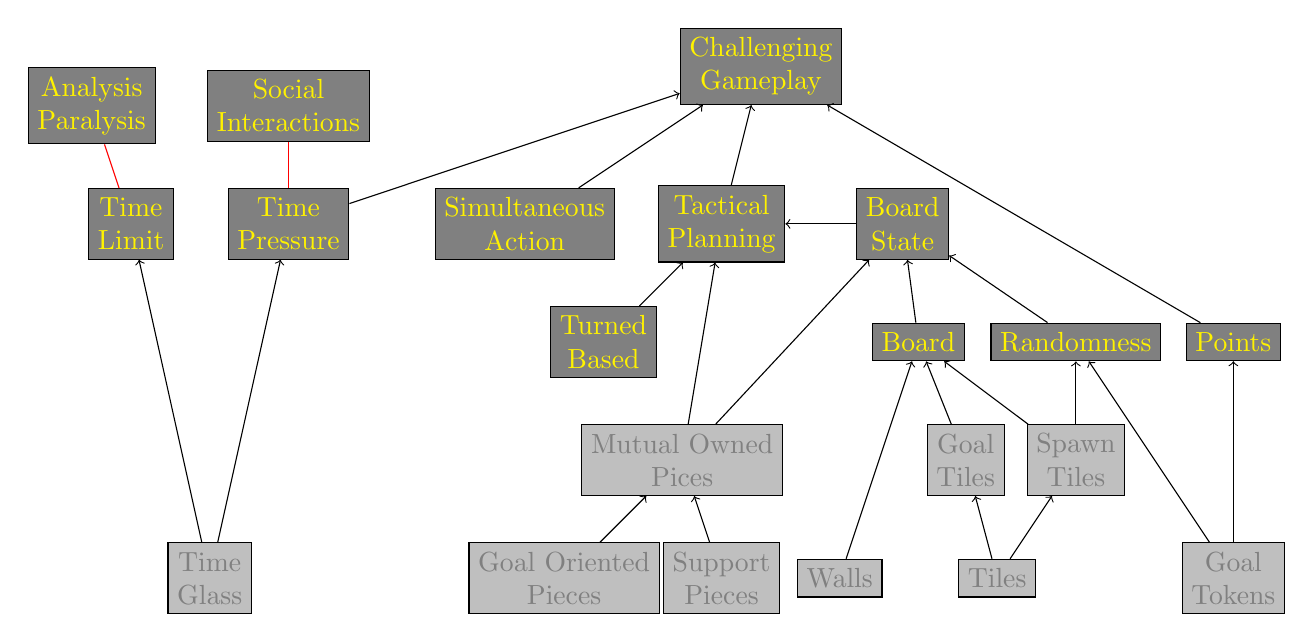
\begin{tikzpicture}

    \node[draw,fill=gray!50,text=gray, align=center] (TiGl) at (-6,0) {Time\\Glass};

    \node[draw,fill=gray!50,text=gray, align=center] (GOPi) at (-1.5,0) {Goal Oriented\\Pieces};
    \node[draw,fill=gray!50,text=gray, align=center] (SuPi) at (0.5,0) {Support\\Pieces};
    
    \node[draw,fill=gray!50,text=gray, align=center] (Wa) at (2,0) {Walls};
    \node[draw,fill=gray!50,text=gray, align=center] (Ti) at (4,0) {Tiles};

    \node[draw,fill=gray!50,text=gray, align=center] (GoTo) at (7,0) {Goal\\Tokens};  

    \node[draw,fill=gray!50,text=gray, align=center] (MOPi) at (0,1.5) {Mutual Owned\\Pices};
    \node[draw,fill=gray!50,text=gray, align=center] (GoTi) at (3.6,1.5) {Goal\\Tiles};
    \node[draw,fill=gray!50,text=gray, align=center] (SpTi) at (5,1.5) {Spawn\\Tiles};

    \node[draw,fill=gray,text=yellow, align=center] (TiLi) at (-7,4.5) {Time\\Limit};
    \node[draw,fill=gray,text=yellow, align=center] (TiPr) at (-5,4.5) {Time\\Pressure};

    \node[draw,fill=gray,text=yellow, align=center] (Bo) at (3,3) {Board};
    \node[draw,fill=gray,text=yellow, align=center] (Ra) at (5,3) {Randomness};
    \node[draw,fill=gray,text=yellow, align=center] (Po) at (7,3) {Points};
    \node[draw,fill=gray,text=yellow, align=center] (TuBa) at (-1,3) {Turned\\Based};

    
    \node[draw,fill=gray,text=yellow, align=center] (AnPa) at (-7.5,6) {Analysis\\Paralysis};
    \node[draw,fill=gray,text=yellow, align=center] (SoIn) at (-5,6) {Social\\Interactions};
    \node[draw,fill=gray,text=yellow, align=center] (SiAc) at (-2,4.5) {Simultaneous\\Action};
    \node[draw,fill=gray,text=yellow, align=center] (TaPl) at (0.5,4.5) {Tactical\\Planning};
    \node[draw,fill=gray,text=yellow, align=center] (BoSt) at (2.8,4.5) {Board\\State};

    \node[draw,fill=gray,text=yellow, align=center] (ChGa) at (1,6.5) {Challenging\\Gameplay};

    \draw[->,draw=black] (TiGl) to (TiLi);
    \draw[->,draw=black] (TiGl) to (TiPr);

    \draw[->,draw=black] (GOPi) to (MOPi);
    \draw[->,draw=black] (SuPi) to (MOPi);

    \draw[->,draw=black] (Wa) to (Bo);
    \draw[->,draw=black] (Ti) to (GoTi);
    \draw[->,draw=black] (Ti) to (SpTi);

    \draw[->,draw=black] (GoTi) to (Bo);
    \draw[->,draw=black] (GoTo) to (Po);
    \draw[->,draw=black] (SpTi) to (Bo);

    \draw[->,draw=black] (SpTi) to (Ra);
    \draw[->,draw=black] (GoTo) to (Ra);
    
    \draw[->,draw=black] (Ra) to (BoSt);
    \draw[->,draw=black] (Bo) to (BoSt);
    \draw[->,draw=black] (MOPi) to (BoSt);
    \draw[->,draw=black] (Po) to (ChGa);
    \draw[->,draw=black] (TiPr) to (ChGa);

    \draw[->,draw=black] (TuBa) to (TaPl);
    \draw[->,draw=black] (MOPi) to (TaPl);
    \draw[->,draw=black] (BoSt) to (TaPl);
    \draw[->,draw=black] (SiAc) to (ChGa);
    \draw[->,draw=black] (TaPl) to (ChGa);

    \draw[-,draw=red] (TiLi) to (AnPa);
    \draw[-,draw=red] (TiPr) to (SoIn);

  \end{tikzpicture}

  \caption{Analysis of Ricocheting Robots using Game Design Pattern. Light gray boxes indicates gameplay mechanics unique to Ricocheting Robots. Dark gray boxes ate abstract mechanics found in other games. Edges with arrows indicate that the pattern being pointed to is instantiated by the other pattern connected to the edge. Red edges indicates that at pattern is in conflict with another pattern.} 
  \label{fig:RRW}
\end{figure}


\subsection{Similarities and difference between the game using our analysis}
  As Figures \ref{fig:A7W} and \ref{fig:RRW} shows there are a lot of similarities between the games.Even though they are different genres and their basic game play do not share any similarities. The main gameplay mechanic is that of the \textit{tactical planning} which is important in both games. In 7 wonders the player has to plan which card by tactical planning and in Ricocheting robots the tactical planning element is how to move and place the robot pieces to reach the goal tile. 

  \paragraph{Another similarity is that both game has been able to avoid \textit{Analysis Paralysis}} by different mechanics. \textit{Analysis Paralysis} is when a player is presented with a couple of options and takes a long time to reach a decision, which makes other players wait to start their player session. As our analysis states 7 wonders have solved this by limit a player's choices due to the \textit{Drafting} mechanic. While Ricocheting robots solves this by having a time limit for a player session. Another mechanic that contributes to this is that the player session takes place simultaneously and therefore limits the waiting time that a \textit{Analysis Paralysis} can cause.

  \paragraph{Randomness and replayability}. In both games randomness is used to give a unique player experience every time. In richocheting robots due to the random order of goal tokens, the random spawn tiles in the set up phase and the shortest path found by a player, are all variables wich makes every game unique. Wich increase the playability of the game. 7 wonders also ralay on this fact for replayability. 

\section{Design structures in the games}
This section answers the questions stated by the excersise. It focus on what gameplay mechanics are used to achive a certain goal. 

\subsection{Keeping players engaged with the game}
\paragraph{Due to 7 Wonders} drafting mechanics players are playing simultaneously. Which in the groups opinion is one of the key components of getting players engaged in the game, which gives minimal waiting time for others to end their player session. Another aspect of 7 wonders drafting mechanics is that players need to analyze opponents board state and base their card pick and overall strategy upon that. Since the board state changes for each picked card there always new information to process. Which helps players to engage more in the game.
Another example as described in section~\ref{sec:thoughtsGP7wond} is when a player gets "the perfect card", the reward of this can get a player more engage. One could argue that this can make the opponents less engaged in the game due to the advantege, but our opinion is that even if a player gets a big advantege the game sessions are so short that other players would not have time to lose interst.  

\paragraph{In Ricocheting Robots} everyone is playing simultaneously often you can not be sure that you have found an optimal solution, therefore a player can always try to find a better solution. Intense Competitive game play due to the time stress. If someone is dominating their opponents, the game session is so short that players are probably not losing their interests.

\subsection{Ending the game in time}
\paragraph{7 Wonders} have a fixed amount of cards to play during each of the three stages of the game. One card is played each round and each stage consists of six rounds.

\paragraph{Ricocheting Robots} ha a limited number of Goal tokens, which regulate the game time. There is a possibility that the game end before all tokens are used, since a player only need to collect a constant number of tokens to win the game.

\subsection{Player interaction}

\paragraph{In 7 wonders} one can not directly interact with all other players, only ones neighbours(players on the left and right side). One can interact with neighbours by either trade gold for resources or beat them in military power. As described in section~\ref{sec:what7wond} nearly all cards have a resource requirements that must be meet to be able to play it. Its very important to watch the neighbours resource stockpile to see if one can use them to pay for a card. The other aspect is military power. At the end of each age of the game, a player's military status is compared to ones neighbours. The one with a higher military status gets a fixed amount of points while the loser of gets a minus point. These points get counted in the \textit{set-down} stage of the game. The number of points is determined by which age the battle is sattle in. The later age, the higher point. 
There are a lot of indirect interaction between all players in 7 wonders, due to the drafting mechanic. Players should always base their picks on what their opponents are picking. For example if someone goes heavy on science cards others need to pick this category or \textit{hate-pick} science cards and use these to build wonders or discarding them for currency.

\paragraph{In Ricocheting Robots} the players are always trying to beat their own or other players solutions, by figure out another one path to the goal using even fewer moves. Wich means that the player interaction is the bread and butter of the game design, since the difficulty of the game is based on cost of the current known best paths, which is always stated by a player.

\paragraph{Overall both games} have a lot of indirect interaction between players. Both the drafting mechanics in 7 wonders and the path finding in Ricocheting Robots are the core gameplay mechanics and they affects the other players indirectly. Based on this our conclusion is that these indirect interaction benefits the games, since it is hard to target a specific player which can make the game unsatisfying.

\subsection{Make the payer achieving something}
\paragraph{7 wonders} gives the player the ability to build a civilisation. Even if the player indirectly are collecting points by building these aspects of the civilisation. When the game ends each players civilisation have made a giant leap in progress then when the game started. 

\paragraph{In Ricocheting Robots} when a player found a path he had achieved something. Even if is not the winning path, a player still has figured out the puzzle.

\section{What parts of the gameplay should be removed from the game or are missing?}
The analysis 


\newpage
\bibliographystyle{apacite}
\bibliography{bib}

\end{document} 



